\graphicspath{{images/mspaper/}}

\chapter{STUDY I: Diffusivity signatures characterize trigeminal neuralgia associated with multiple sclerosis}
\chaptermark{Study I}
\label{section:study1}

This study was published in Multiple Sclerosis Journal \textcopyright 2016:

\bibentry{Chen2016a}


\section{Abstract}
\textbf{Background: }Trigeminal neuralgia secondary to multiple sclerosis (MS-TN) is a facial neuropathic pain syndrome similar to classic trigeminal neuralgia (TN). While TN is caused by neurovascular compression of the $5\textsuperscript{th}$ cranial nerve (CN V), how MS-related demyelination correlates with pain in MS-TN is not understood. 

\textbf{Objectives: }We aim to examine diffusivities along CN V in MS-TN, TN and controls in order to reveal differential neuroimaging correlates across groups.

\textbf{Methods: }3T MR diffusion weighted, T$_{1}$, T$_{2}$ and FLAIR sequences were acquired for MS-TN, TN, and controls. Multi-tensor tractography was used to delineate CN V across cisternal, root entry zone (REZ), pontine, and peri-lesional segments. Diffusion metrics including FA, RD, AD and MD were measured from each segment. 

\textbf{Results:} CN V segments showed distinctive diffusivity patterns. The TN group showed higher FA in the cisternal segment ipsilateral to the side of pain, and lower FA in the ipsilateral REZ segment. The MS-TN group showed lower FA in the ipsilateral peri-lesional segments,  suggesting differential microstructural changes along CN V in these conditions. 

\textbf{Conclusions:} The study demonstrates objective differences in CN V microstrucuture in TN and MS-TN using non-invasive neuroimaging. This represents significant improvement in the methods currently available to study pain in MS. 

\section{Introduction}
Trigeminal neuralgia is a neuropathic pain disorder characterized by severe, lancinating, facial pain with no major clinical sensory deficits. The pain occurs in one or more territories of the branches of the 5th cranial nerve (CN V) and is often triggered by innocuous stimuli, such as a light touch to the face. Classic trigeminal neuralgia is presumed to occur as a result of neurovascular compression at the root entry zone (REZ) of CN V (also referred as ‘idiopathic’; henceforth referred to simply as TN)(M Hodaie \& Coello, 2013). TN pain symptoms can also occur secondary to multiple sclerosis (MS-TN), where MS patients have a 20-fold risk of developing TN pain than the general population (up to 0.1\%) \cite{VanHecke2014}. 
While experientially similar, the pathophysiology of MS-TN differs from TN and involves CNS demyelination \cite{lazar1979trigeminal,Nurmikko2009}. The manner in which CNS demyelination results in pain is unclear. Brainstem plaques can be common in MS, but not all MS patient with brainstem plaques suffer from MS-TN. Furthermore, the presence of bilateral plaques does not clearly correlate with bilateral MS-TN pain \cite{DeSanti2011a,Love2001a}, highlighting the complex and uncertain relationship between the presence of plaques and pain\cite{DaSilva2005}. Importantly, this also highlights the fact that conventional MR plaque visualization does not fully correlate with MS clinical symptoms or their severity, and so improved neuroimaging methods are needed \cite{Seixas2014}. As classic TN is most commonly associated with vascular compression at the trigeminal nerve root entry zone, it is possible that in some MS patients neurovascular compression can also be present, adding further complexity to the diagnosis and treatment of trigeminal pain \cite{Sandell2010e}.

Understanding the microstructural anatomy of the trigeminal fibres is essential to determine how MS affects CN V brainstem fibres and how alterations to CN V in MS are related to the clinical presentation of pain. Direct comparisons between TN and MS-TN at the level of CN V brainstem fibres has been challenging because it is difficult to reliably identify, segment, and measure trigeminal anatomy with conventional magnetic resonance imaging (MRI)(Figure 1A-B) \cite{Cruccu2009,DaSilva2005}. Conventional MR imaging cannot visualize in isolation the brainstem fibres of CN V. Furthermore conventional tractography cannot resolve the brainstem crossing fibres \cite{Farquharson2013}, which leads to unreliable CN V delineations within the brainstem, and inaccuracies in diffusivity measurements. 

Diffusion tensor imaging (DTI) metrics, based on estimating the Gaussian diffusion of water in the neural tissue, can provide important insights to microstructural neural tissue changes in both pathological and normal states. Metrics including fractional anisotropy (FA), and radial (RD), axial (AD), and mean diffusivities (MD), reflect diffusivity change measured as a parameter of the estimated Gaussian diffusion tensor eigenvectors.  FA reflects the shape of the ellipsoid Gaussian tensor as a measure of anisotropy, and is correlated with both structural and cognitive changes that follow adverse brain changes such as traumatic brain injury, aging and Alzheimer’s disease \cite{Bendlin2008,Charlton2006,Kinnunen2011c,Mielke2012}. RD is a measure of the cross-sectional diffusion as an average of the second and third diffusion eigenvalues, and has been shown to positively correlate with axonal demyelination \cite{Song2002,Song2005}. AD is the greatest diffusion eigenvalue and has been positively correlated with axonal degeneration \cite{Budde2009,Song2002}, and MD is the mean of all three diffusion eigenvalues and is related to the increase in tissue inflammation and edema \cite{Beaulieu2002}. In MS studies, FA, RD and MD appear abnormal in or near MS lesions. The changes in diffusivity alter the Gaussian tensor profile and results in decreased FA, increased RD and increased MD \cite{Braley2012,Janve2013,Klawiter2011,Lin2007,Senda2012g}. While AD is generally not correlated with demyelination \cite{Song2002}, there have been findings associating decreases in AD with the presence of neurological damage in MS \cite{Budde2008,Kim2006}. 

The major technical limitation of diffusion tractography to date has been the inability of resolving crossing fibres using a single tensor Gaussian diffusion model \cite{Farquharson2013}, which has proved unsuitable for the visualization of brainstem tracts. However, techniques that use high angular resolution imaging  with an increased number of gradient directions acquired during diffusion weighted imaging (DWI), and advances in multi-tensor tractography (MTT) have improved the ability to delineate fibres in brain regions that have dense fibre crossings, such as the brainstem \cite{DellAcqua2007,Descoteaux2009c,Fillard2011,Qazi2009}. The microstructure of CN V in TN has recently been shown to be abnormal in terms of DTI metrics in the trigeminal REZ \cite{Desouza2013}. DTI metrics, as correlates of microstructural anatomy, are also important in identifying the nerve in pain in TN\cite{Hodaie2009a}. 

In this study of MS-TN, we hypothesize that A) myelination correlates of the trigeminal brainstem fibres, assessed with diffusion metrics, will reveal a pattern which is unique to MS-TN, despite inherent differences in precise lesion location, and B) diffusion metrics along the nerve will help differentiate between TN, MS-TN and healthy subjects, and may in future serve as a neuroimaging signature of pain in these populations. 
We used MTT and diffusivity metrics to identify specific neuroanatomical diffusivity differences between TN and MS-TN. Specifically, our aims were: 1) Visualize the isolated tracts of brainstem trigeminal fibres using MTT; 2) Sample and compare CN V diffusivities in MS-TN between symptomatic (+) and asymptomatic (-) sides of a) CN V at the REZ, b) brainstem CN V segments unaffected by MS plaques, and c) brainstem CN V segments with the presence of MS plaques; 3) Contrast diffusivity findings with CN V diffusivities in TN patients, MS-TN patients and healthy controls.

\section{Methods}

Magnetic resonance images were acquired using GE Signa HDx 3T scanner with an 8 channel head-coil. MR sequences were acquired from 3 groups (n=10 in each): unilateral MS-TN (4 males, 6 females; mean age  $53\pm8.6$ years) with no evidence of neurovascular compression of CN V at the REZ, unilateral TN (3 males, 7 females; mean age $57.1\pm8.5$ years), and healthy controls (3 males, 7 females; mean age $55.8\pm7.4$ years). Clinical pre-screening of MS patients and their associated lesion locations were performed using T$_{2}$ and FLAIR sequences. However clinical T$_{2}$ slice thickness was too large (\textgreater 3 mm) for proper assessment of 3D lesion volume. Therefore once the lesion was identified, the fast spoiled gradient echo (FSPGR) T$_{1}$ anatomical image was registered to the diffusion image in order to localize the MS lesion across multiple modalities for ROI placement. DWIs were acquired with 1 B$_{0}$ scan, 60 gradient directions, 3mm slice thickness and in-plane resolution of 0.9375$\times$0.9375 mm, b$_{0}$=1000 s/mm$\textsuperscript{2}$, TE=88.6 ms, TR=17000 ms, flip angle=90 deg, matrix=128$\times$128. T$_{1}$ FSPGR anatomical scans were acquired with 1mm slice thickness and in-plane resolution of 0.9375$\times$0.9375mm, slice spacing=1 mm, TE=5.052 ms, TR=11.956 ms, flip angle=20 deg, field of view (FOV)=240 deg, matrix=256$\times$256. T$_{2}$images were acquired with 4mm slice thickness, in-plane resolution=0.4297$\times$0.4297 mm, TE=94.14 ms, TR=5200 ms, flip angle=90 deg, FOV=170 deg, matrix=512$\times$512. FLAIR images were acquired with 4mm slice thickness, in-plane resolution=0.4297$\times$0.4297 mm, TE=141.4 ms, TR=8652 ms, flip angle=90 deg, FOV=220 deg, matrix=384$\times$224.

Images were analyzed with 3D Slicer (NA-MIC©, http://www.slicer.org) \cite{Pieper2004}. DWI sequences were corrected for eddy-current and motion distortions with appropriate corrections to gradient vectors, and imported into 3D Slicer for single-tensor diffusion tractography (SDT), where tracts were generated with initial seed spacing=0.5 mm, initial seeding FA threshold=0.2, stopping FA threshold=0.1, curvature threshold=0.8 and integration distance=0.1. Region-of-interests (ROI) seeding points were generated at a spacing of 0.25mm, or 64 points per voxel; MTT propagations were initiated at C1 threshold=0.2, tensor fraction=0.2, curve radius=0.8 rad, minimal length=10 mm, step size=1 mm. T$_{1}$ anatomical images were registered to the DWI using rigid transformation. To generate CN V tractography, ROIs were placed bilateral at the CN V at the REZ, and were used for both SDT and MTT. 

Diffusion parameters (FA, AD, RD, MD) were measured from 4 sets of pre-defined bilateral ROIs (Figure~\ref{fig:MSfigure1}C-D). Cross-sectional areas were based on tractography delineations, and thickness of 2 voxels. Location of the ROIs were defined based on trigeminal anatomy: 1) The cisternal ROI is measured from the nerve segment situated within the cisternal space surrounding the pons, at the mid-point between the Gasserian ganglion and the root entry zone; 2) the REZ ROI is defined at the junction where the CN V crosses from the cisternal space into pontine brainstem. This is where the neural myelination transitions from peripheral myelination (Schwann cells) to central myelination (oligodendrocytes). The ROI must include the cisternal segment and pontine segment at the transitional zone; 3) the pontine ROI is defined in the intra-pontine CN V segment at the mid-point between the REZ and the trigeminal nucleus. In MS-TN patients it is defined as the mid-point between the peri-lesional ROI and the REZ along the nerve that is not visually affected by any MS lesions (and note that subjects with MS lesions that did not allow ROI placement with at least 2 voxel spacing from peri-lesional and REZ ROIs were excluded as confounders); and 4) the peri-lesional ROI is defined as the intra-brainstem CN V segment at the closest proximity to MS lesions in its vicinity. In TN and control subjects, the corresponding ROI was the nerve segment closest in proximity to the trigeminal nucleus. In these patient groups, the pontine and peri-lesional areas are referred to as distal and proximal brainstem ROIs, respectively. 

Statistical analysis were performed using R statistics software suite(R Development Core Team, 2012). Segments and diffusivity measurements were analyzed separately. Patient group is considered an independent and between-subject factor; symptomatic and asymptomatic sides within the same patient are considered within-subject measures; in controls, the mean measures of left/right sides are used for comparison against other groups. A linear mixed model \cite{Pinheiro2011} is used to determine the statistical significance of within- and between-subject effects. Post hoc analyses were performed using pair-wise Student’s t-test, where multiple comparisons are corrected with false discovery rate correction \cite{Hothorn2008}. Statistical results were plotted \cite{Hunter2007} as diffusivity difference estimate matrices between anatomical regions and different subject groups. Values are mapped as red/blue based on mixed linear regression estimates. Positive estimates, where the group diffusivity parameter is greater in the vertical axis versus the horizontal axis are in red, and negative coefficients are in blue. 


\begin{figure}[p]
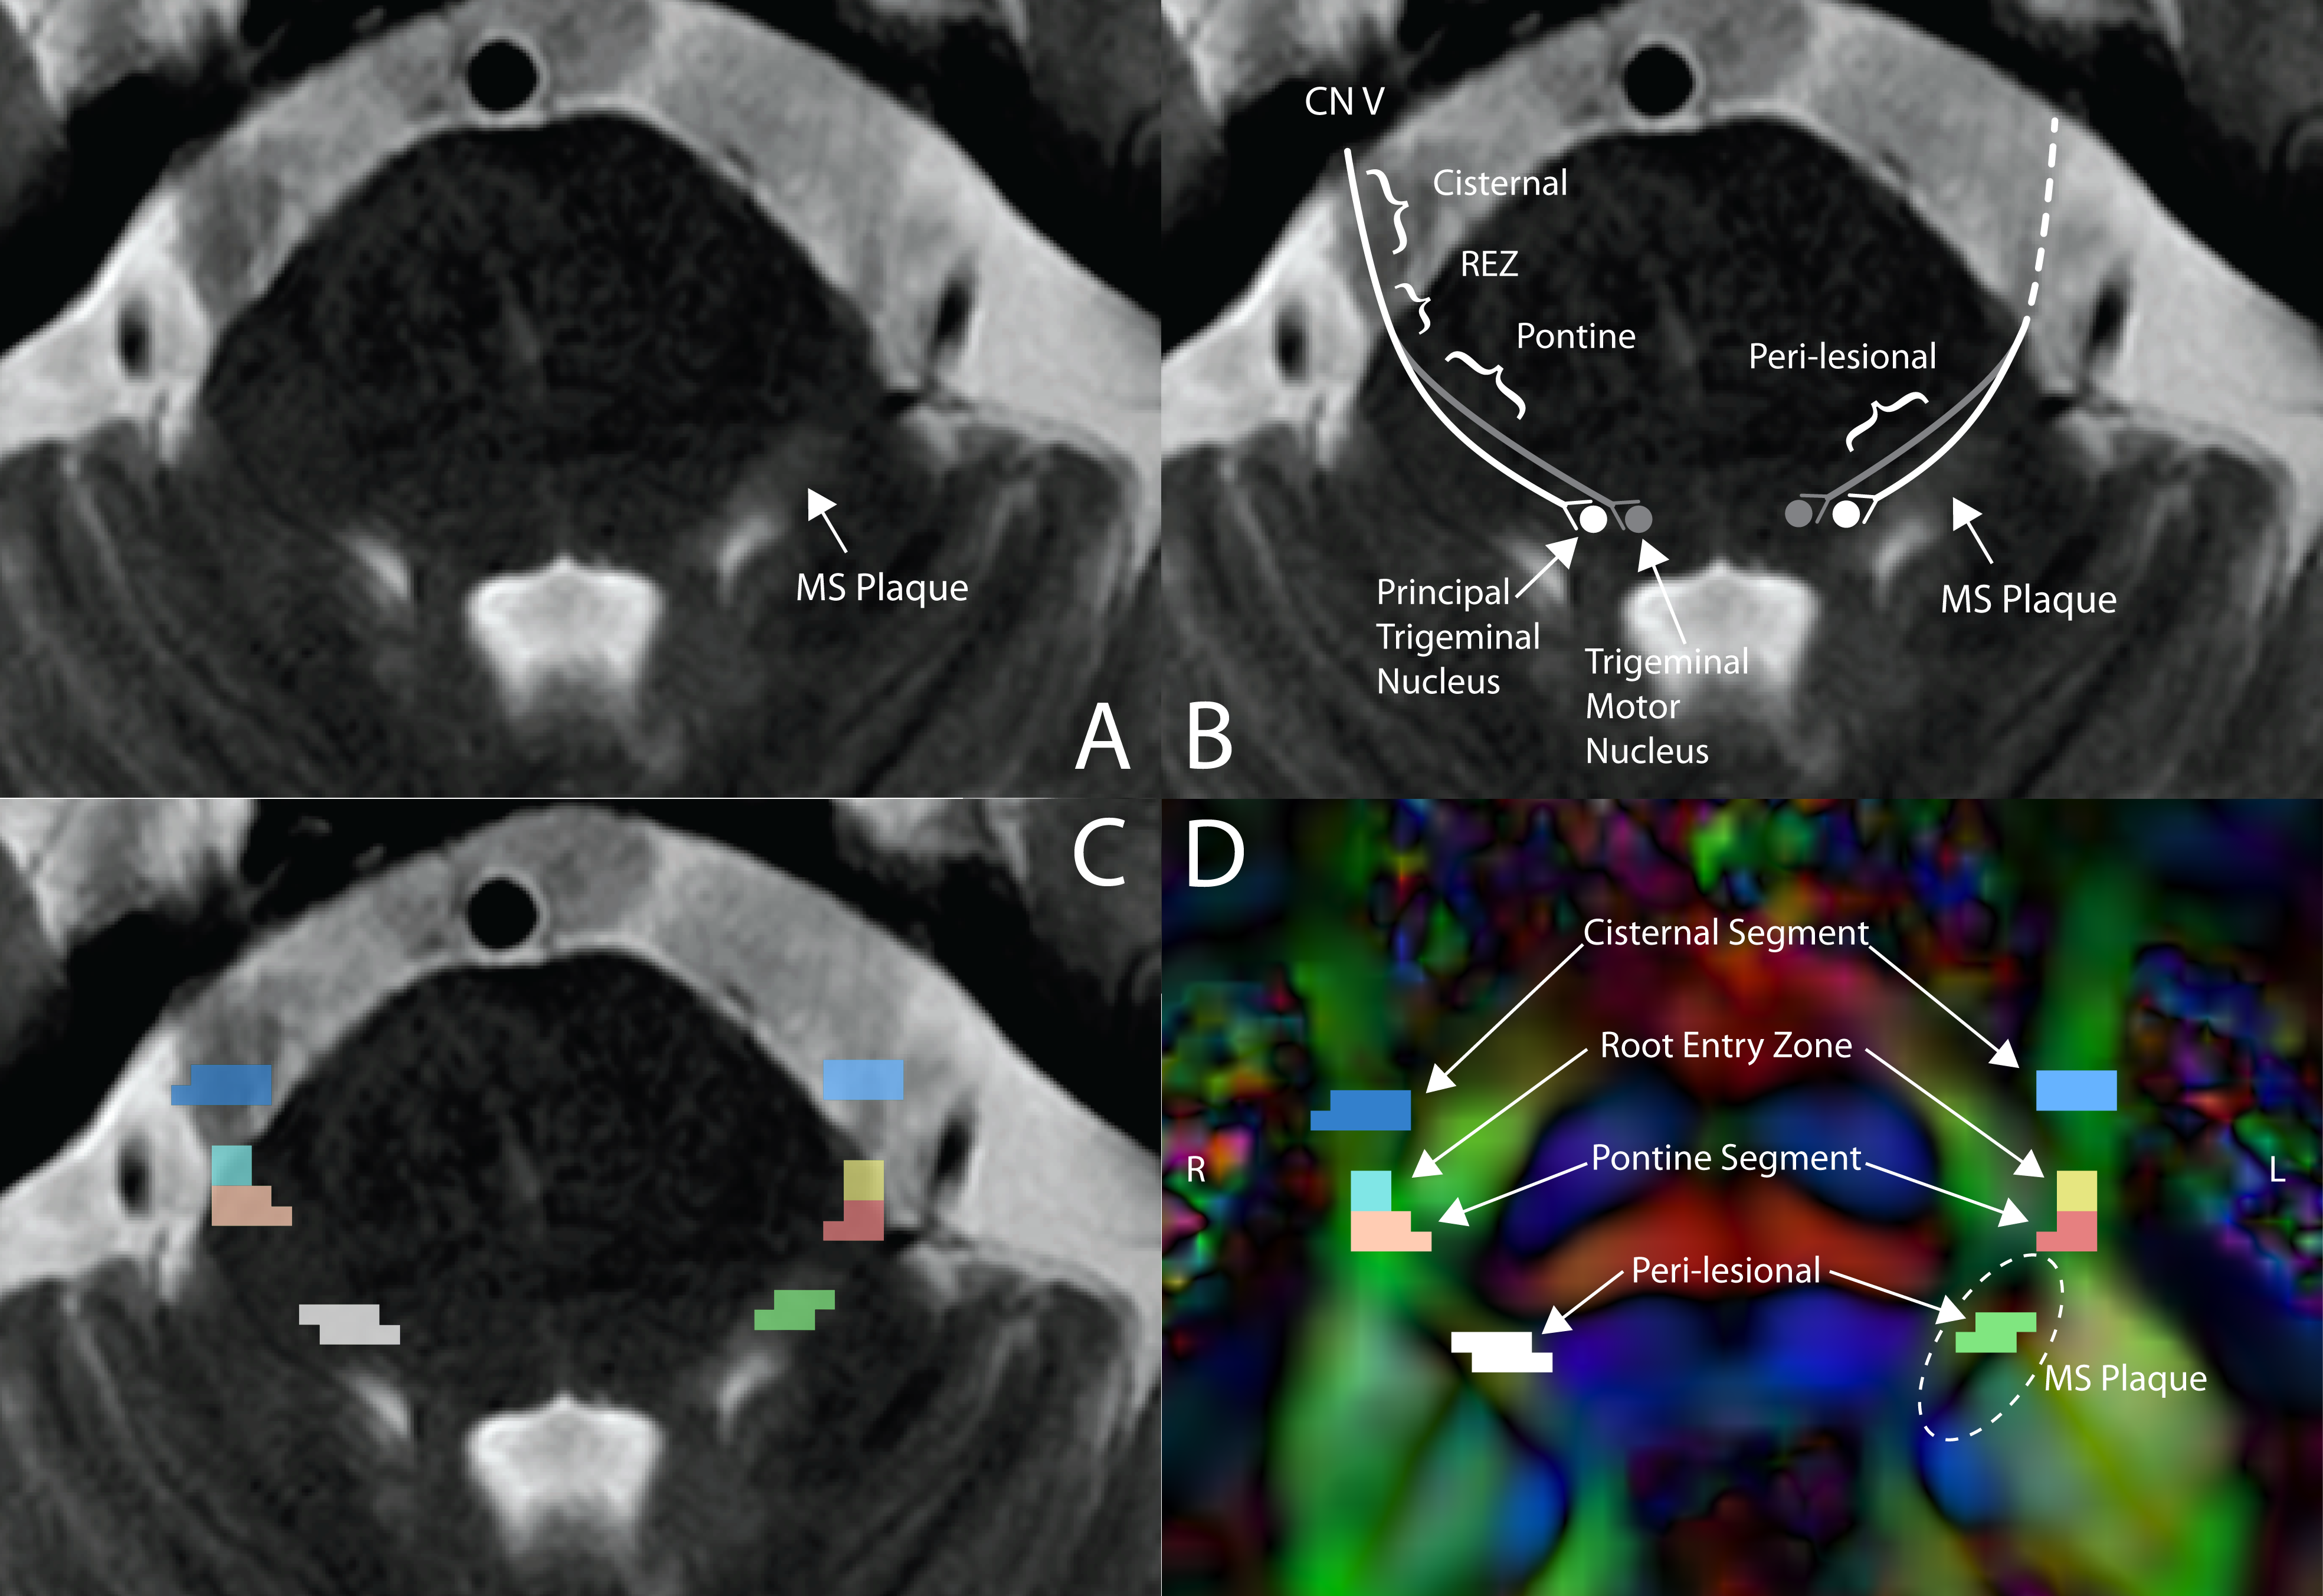
\includegraphics[width=\textwidth]{figure1.png}
\caption[Figure shows the MR images of a typical MS-TN patient at the level of pons.]{Figure shows the MR images of a typical MS-TN patient at the level of pons. The presence of MS plaque in the CNS at the level of trigeminal nerve is characteristic of MS-TN (panel A). Panel B shows the expected course of the trigeminal nerve (CN V) as it synapses onto the principal trigeminal and motor trigeminal nuclei. Note that the exact anatomical relationship between the MS plaque and CN V in this instance cannot be clearly discerned in T2 due to the lack of contrast between the nerve and the surrounding tissue (panels A,B,C). Panels C and D show the placements of the ROIs along the CN V nerve bilaterally in order to measure diffusivity statistics, overlaid with the axial anatomical/ DTI image. The colours of the DTI image are rendered as colour-by-orientation, where by convention red represents left–right, greens represents anterior–posterior and blue represents inferior–superior orientations. Diffusion statistics were measured from four groups of regions: cisternal segment, root entry zone (REZ), pontine, and peri-lesional, as illustrated. Analogous regions in TN patients and controls were similarly placed. Care was taken to differentiate pontine and peri- lesional ROIs in order to measure lesioned and unlesioned regions.}
\centering
\label{fig:MSfigure1}
\end{figure}


\section{Results}
\subsection{MTT permits visualization of brainstem trigeminal fibres}
MTT allowed for the visualization of brainstem CN V fibres in isolation, by distinguishing them from the surrounding crossing cerebellar peduncular fibres. The SDT method could not adequately delineate the nerve (Figure 2). Comparison of tractography results between SDT and MTT showed that SDT was unable to differentiate fibres crossing the cerebellar peduncle fibres, while MTT delineated the brainstem course of CN V into the region of the trigeminal main sensory nucleus. Delineation of MS-TN CN V by MTT revealed that the tracts became visibly sparse as they came into proximity of the MS plaque (Figure 3A). FA decreases in proximity to the MS plaque could also be visualized by colour shift in the tractography model with more orange/yellow colour presented. The fibres of the unaffected CN V did not exhibit this change, and extended caudally into the trigeminal nuclei (Figure 3B). 

\begin{figure}[p]
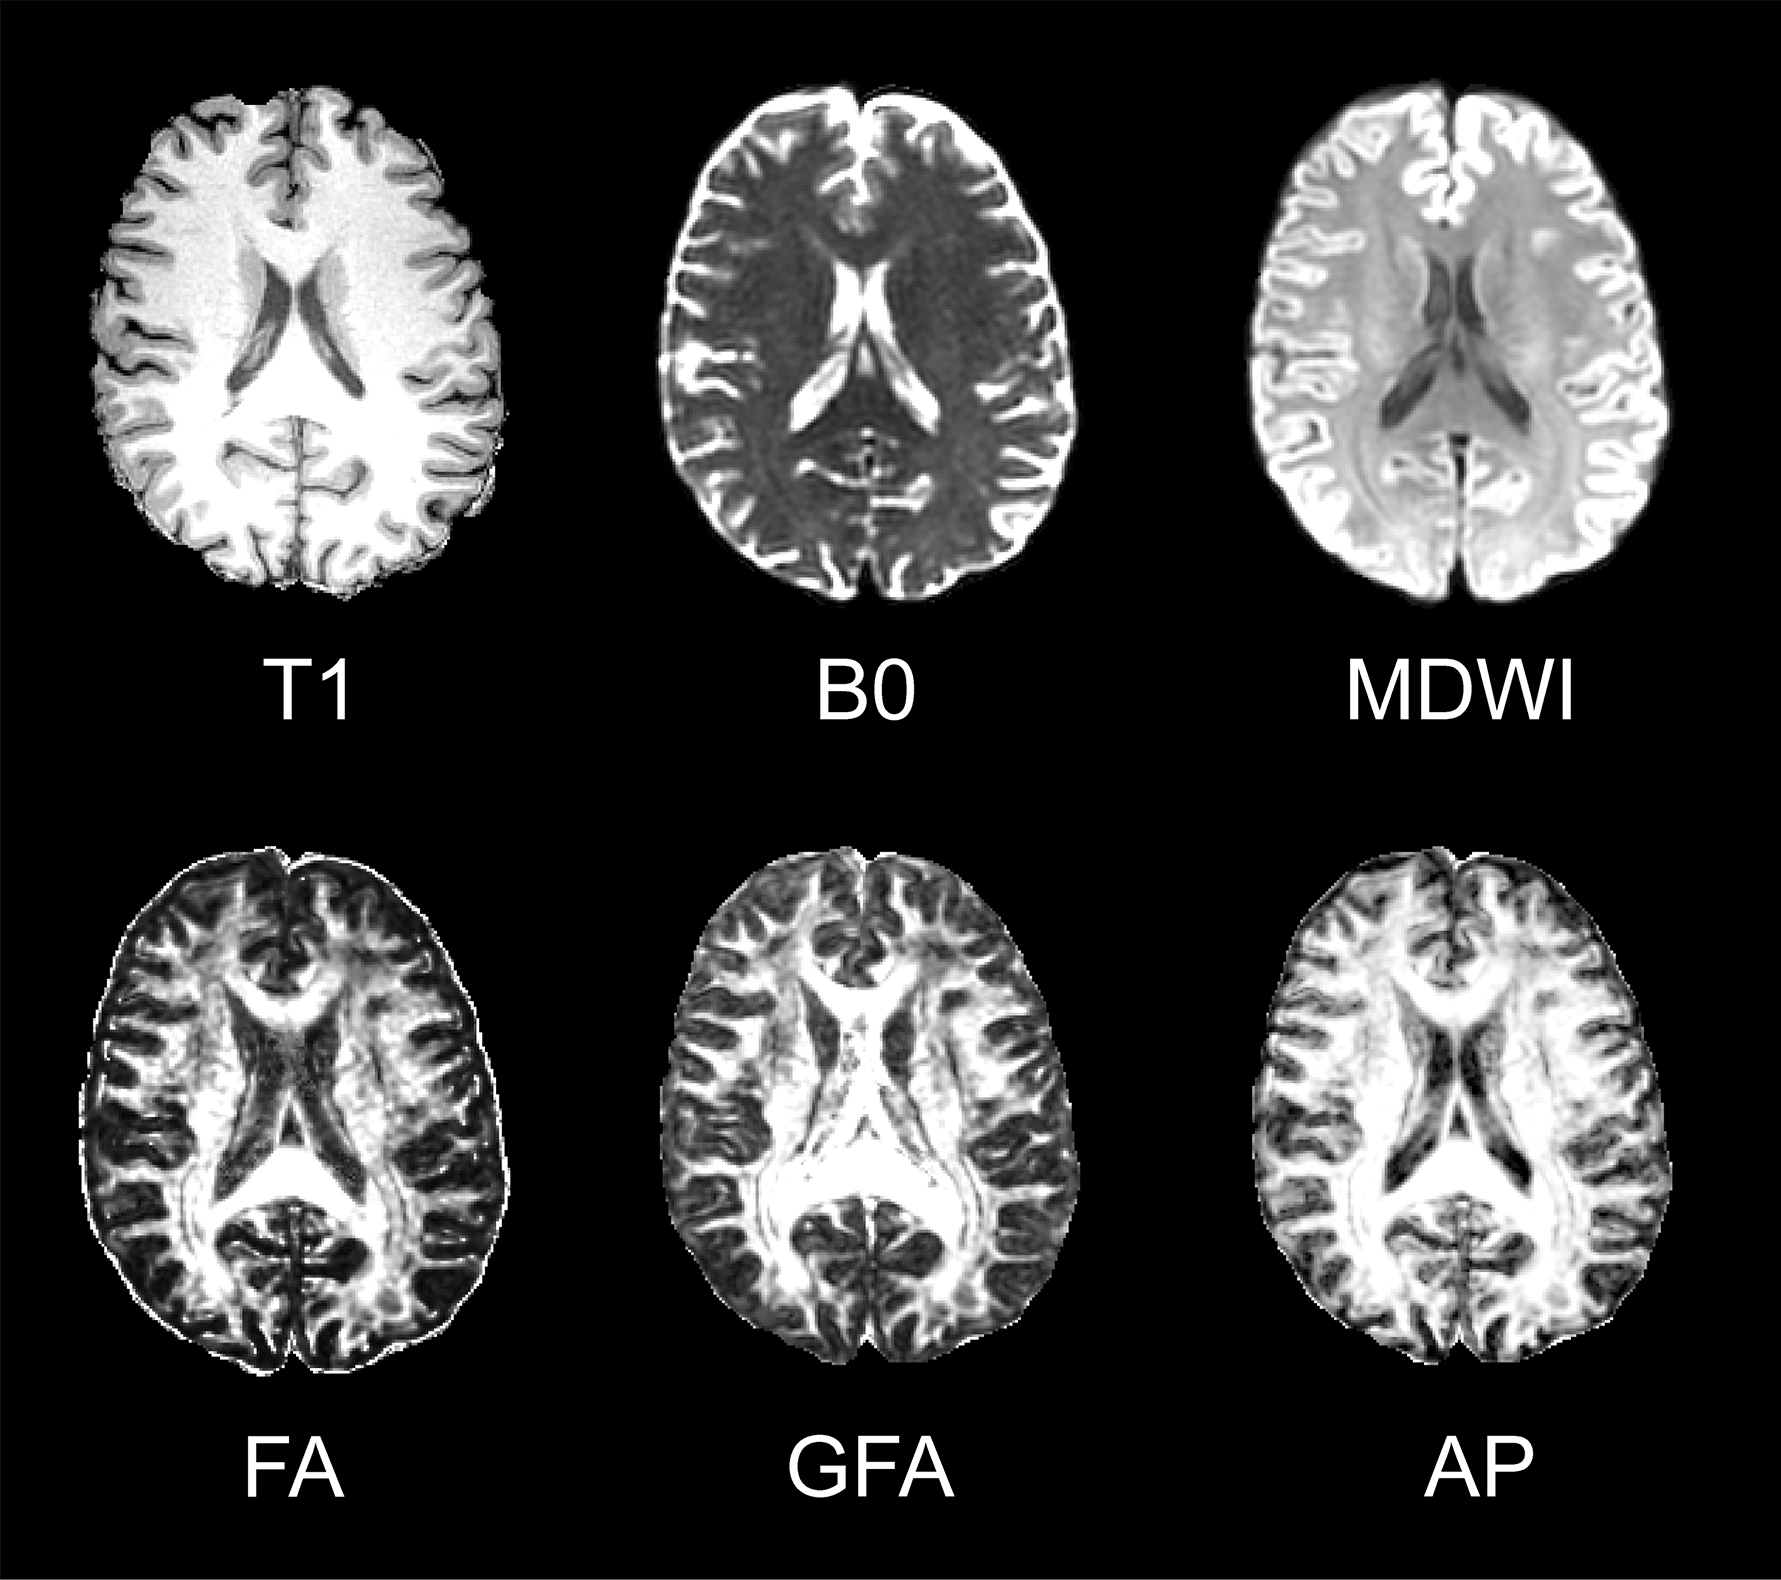
\includegraphics[width=\textwidth]{figure2.png}
\caption[Reconstruction of the trigeminal nerves at the level of pons from a single healthy subject in superior axial views.]{Reconstruction of the trigeminal nerves at the level of pons from a single healthy subject in superior axial views. The reconstructed tracts are overlaid onto the axial DTI/anatomical images. The colours of the underlying scan are rendered as colour-by-orientation, where by convention red represents left–right, greens represents anterior–posterior and blue represents inferior–superior orientations. The colours of the tractography fibres represent the spectrum values of FA (0 to 1), as shown by the legend at the top right corner. Panel A shows that SDT tractography delineated the cerebellar peduncle fibres, but cannot distinguish the brainstem trigeminal fibres (yellow arrows). Red arrows denote the starting point of tract generation for both SDT and MTT methods. Panel B shows that MTT tractography visualized CN V as it coursed through the brainstem towards the trigeminal main sensory nuclei.}
\centering
\label{fig:MSfigure2}
\end{figure}

\begin{figure}[p]
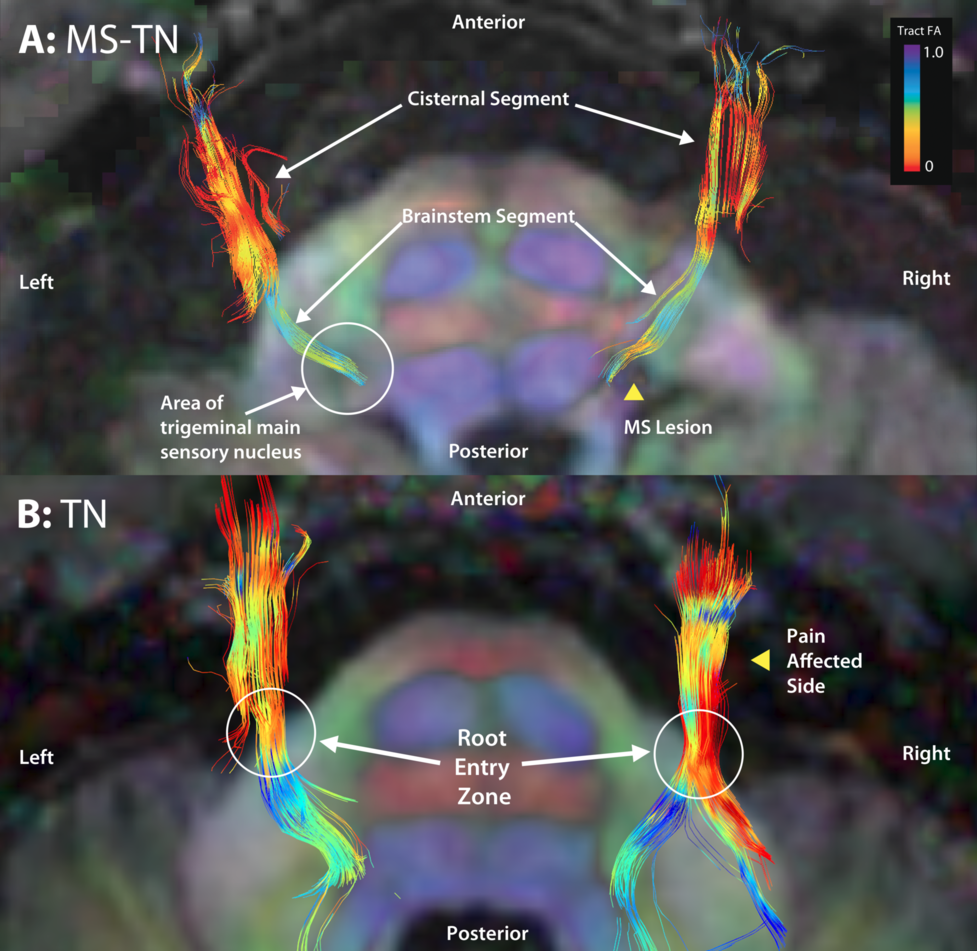
\includegraphics[width=\textwidth]{figure3.png}
\caption[Comparison of tractography delineation between affected and unaffected CN V nerve in the region of the trigeminal main sensory nucleus using the MTT method.]{Comparison of tractography delineation between affected and unaffected CN V nerve in the region of the trigeminal main sensory nucleus using the MTT method. Images are shown in superior axial view. Panel A shows the MS-TN tractography delineations. There is focal decrease in CN V FA in the region of the MS lesion (yellow arrow). Panel B shows the TN tractography delineations, where there is no such FA decrease in the brainstem segment. Please refer to Figure \protect\ref{fig:MSfigure2} for explanations of colour scales and figure annotations.}
\centering
\label{fig:MSfigure3}
\end{figure}


\subsection{TN and MS-TN are characterized by specific diffusivity signatures}
The resulting coefficient matrices demonstrated unique patterns of diffusion metrics across subject groups in each of the CN V segments measured. Each nerve segment is studied separately, and differences in regional diffusivities were examined in both intra-subject comparisons between symptomatic and asymptomatic sides, as well as inter-subject comparisons between subject groups. The details of the examinations are described as follows:

\subsubsection{Cisternal changes are unique in TN}
In the cistern segment (Figure 4), statistically significant differences are found only between the TN group and other groups. No significant differences were found in between segments of other subject groups. Specifically, the FA measure of symptomatic side (+) in TN patients is shown to be significantly greater compared to all of the other patient groups and segments, while the asymptomatic side (-) in TN patients does not show any significant differences compared to other groups. In RD, AD and MD measurements, the only significant differences are observed between TN(+) and TN(-), where TN(+) RD/AD/MD are lower than that of TN(-). No symptomatic/asymptomatic (+/-) or left/right differences were observed in MS-TN and control groups. These results suggest that the cisternal CN V diffusivity changes are unique to the TN group. 

\subsubsection{REZ changes are found predominantly in TN}
In the REZ (Figure 5), statistically significant results are found within, but not unique to TN. TN(+) FA is shown to be significantly lower than TN(-) FA, while TN(+) RD and MD are shown to be significantly greater than TN(-); TN(+) MD and RD are shown to be significantly greater compared to all other groups and sides; while TN AD showed no significant differences. In contrast, MS-TN patients showed no significant differences between MS-TN(+) and MS-TN(-) sides in any of the diffusivity metrics, suggesting no intra-group differences. Comparisons between MS-TN(+/-) and TN(+/-) revealed no significant inter-group FA differences. However, both TN and MS-TN groups are shown to be different from controls. Both TN(+/-) and MS-TN(+/-) REZ have significantly lower FA than that of control REZ; control AD and RD are shown to be significantly lower than TN(+/-); while there is no significant difference between left and right sides in controls. 
\subsubsection{Pontine diffusivities showed no significant changes in all groups}
In the pontine tissue (Figure 6), there are no significant intra-group or inter-group differences in FA, RD and MD for all groups and sides. However MS-TN(-) AD is significantly higher than TN(+/-) and controls. No intra-group AD differences were found in MS-TN.
2D. Diffusivities in peri-lesional trigeminal fibres highlight MS-TN pain

In the peri-lesional region (Figure 7), the patterns shows significant intra-group and inter-group differences in MS-TN. MS-TN(+) FA is significantly lower than that of MS-TN(-), as well as significantly lower than TN(+/-)and Controls, while MS-TN(-) FA showed no inter-group differences with TN and Controls. RD, and MD showed only intra-group differences between MS-TN(+) and MS-TN(-),where MS-TN(+) RD and MD are significantly higher than that of MS-TN(-). AD showed no significant differences. The pattern of differences for peri-lesional region is unique to MS-TN. 

\begin{figure}[p]
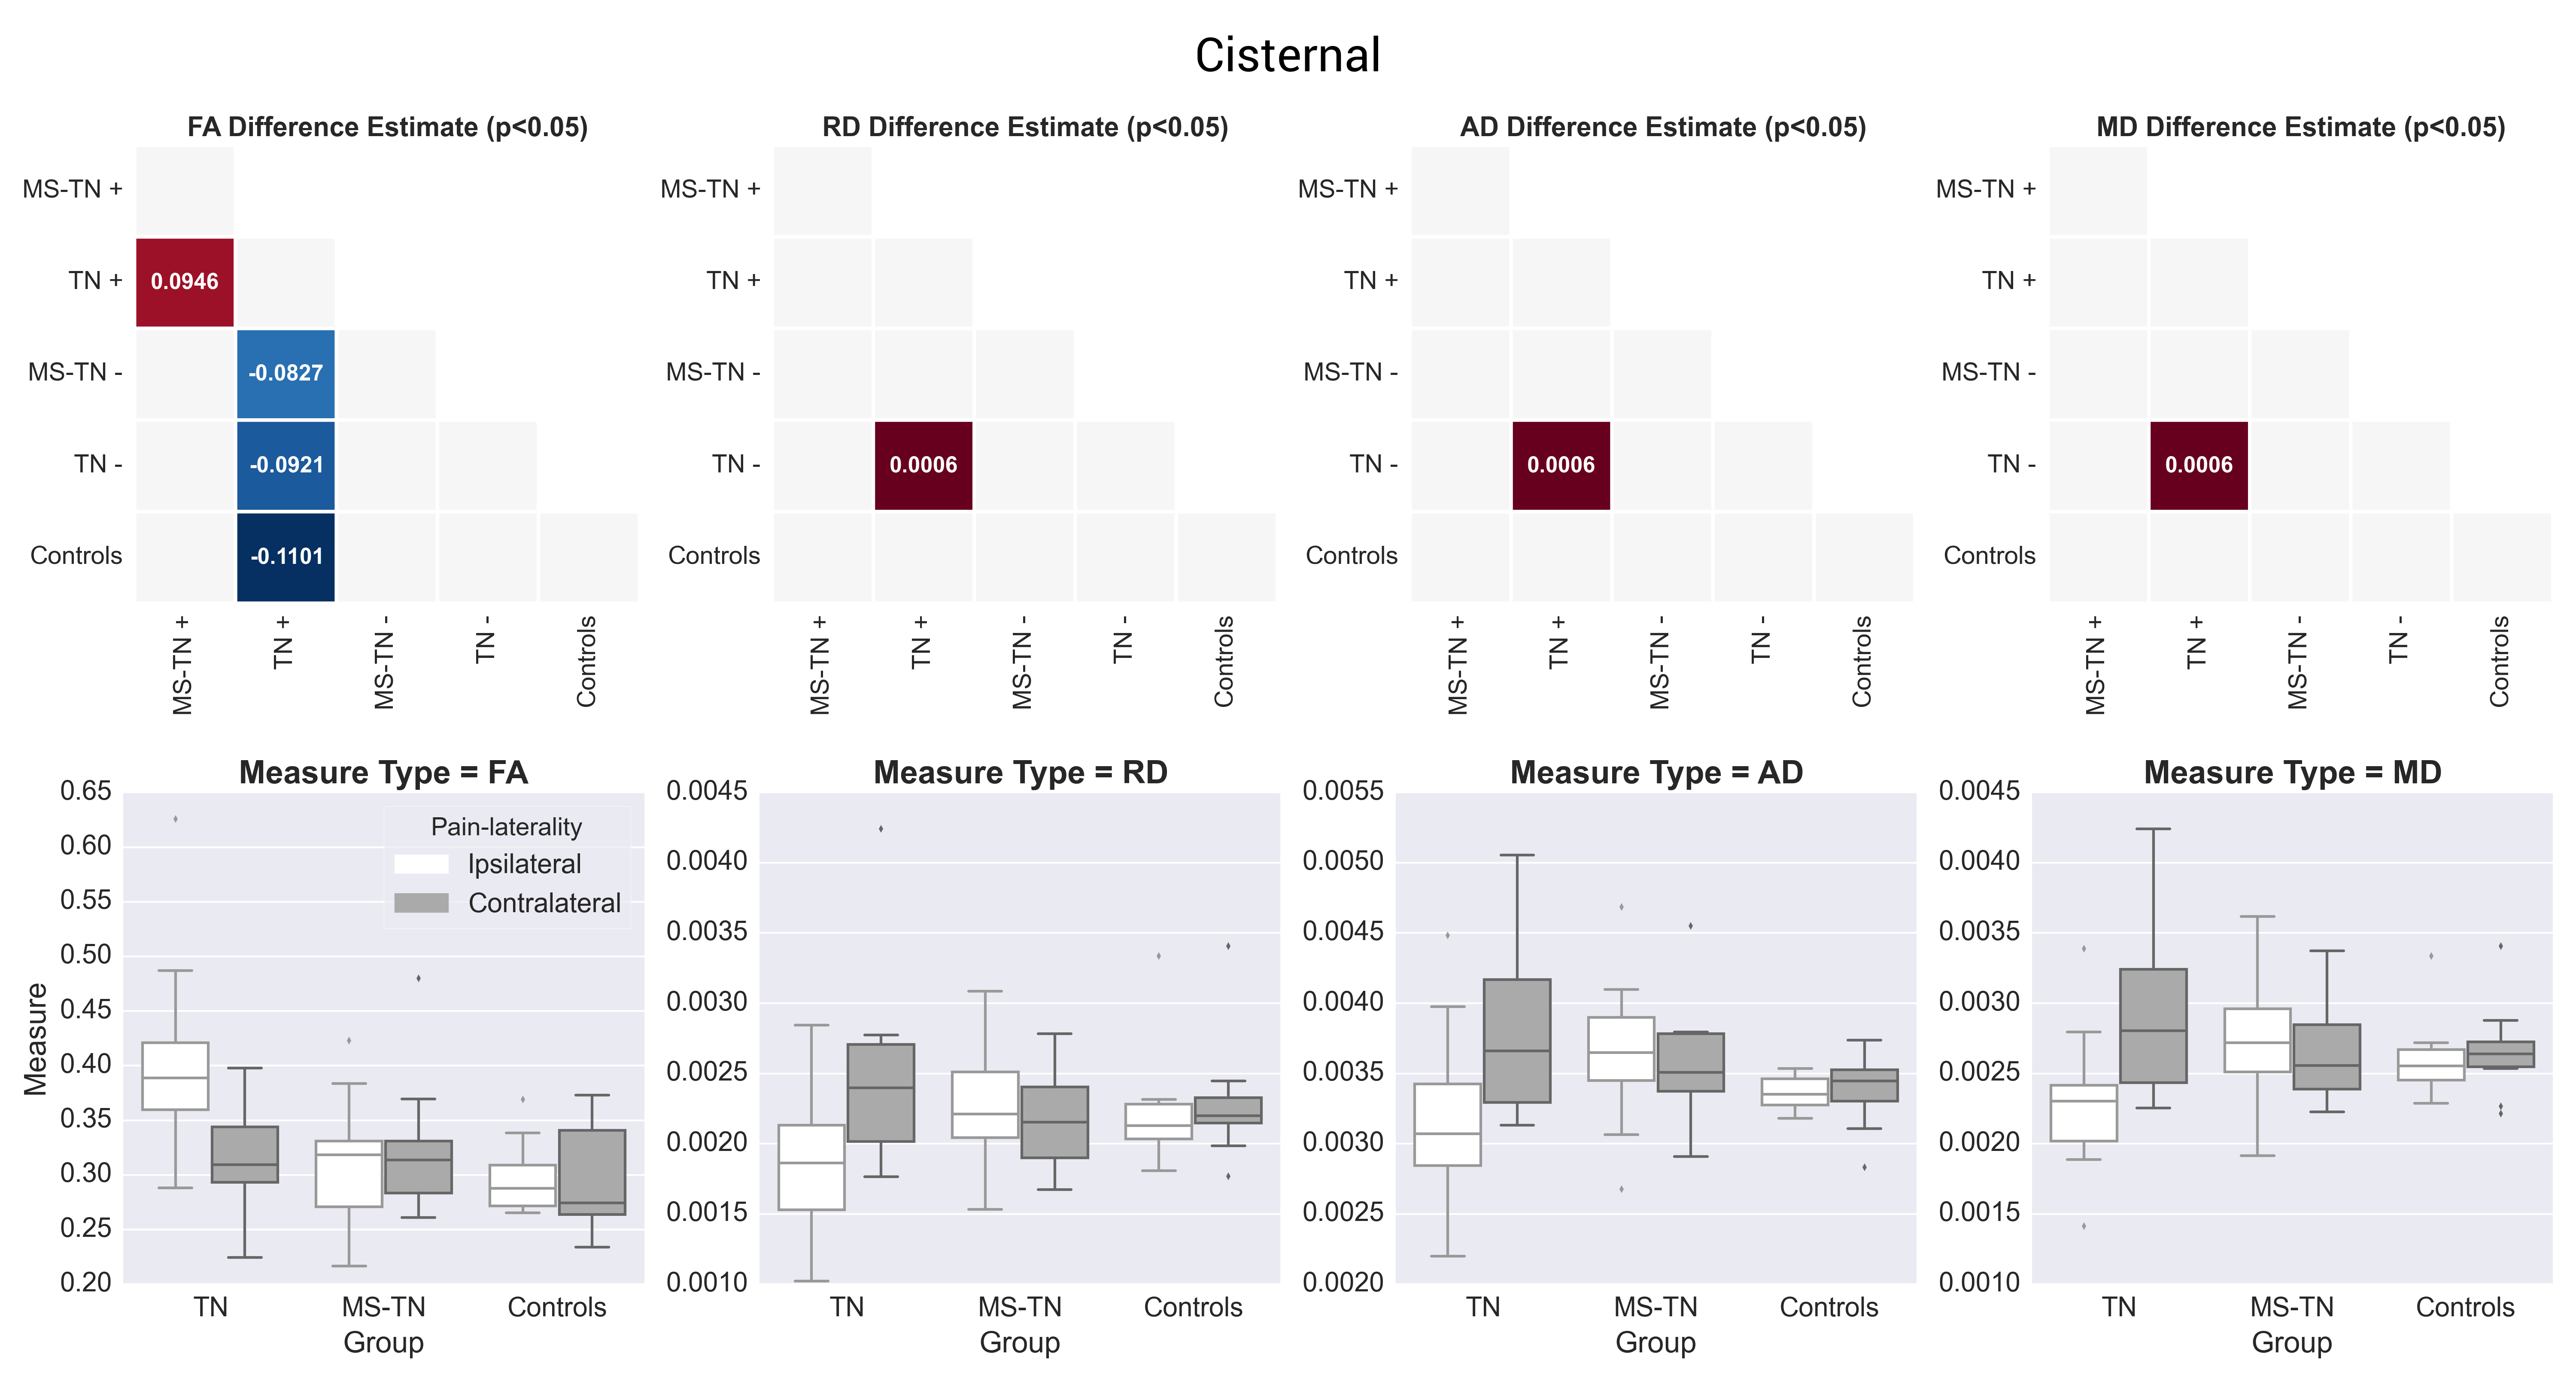
\includegraphics[width=\textwidth]{figure4.png}
\caption[Diffusivity difference estimate matrices of the Cisternal ROIs demonstrating significant differences in regional diffusivities between MS-TN patients, TN patients and controls.]{Top row: Diffusivity difference estimate matrices of the Cisternal ROIs demonstrating significant differences in regional diffusivities between MS-TN patients, TN patients and controls. coloured squares indicate statistically significant differences (p\textless 0.05) after correcting for multiple comparisons with false discovery rate. The (+/-) sign indicate symptomatic (+) and asymptomatic (-) sides of the subject group. The matrix should be read as ‘Y axis in relation to X axis’—for example, A red square indicates that the vertical axis measure (e.g. TN+, the affected side in TN patients) is significantly higher than that of the horizontal axis measure (e.g. MS-TN+, the affected side in MS-TN patients); blue indicates that the measure is lower. The number within the square indicates relative estimated differences. Bottom row: Box-plots of the diffusivity distributions. Note that the control group does not have pain lateralities, therefore ipsilateral indicate the right side in the control group in this figure. The mean of the left-right diffusivities in controls were used for comparisons against other groups. The analysis highlights TN+ specific diffusivity differences in the Cisternal segment of the trigeminal nerve. Specifically TN+ has significantly higher FA than all the other groups, and that there are significant differences between TN+ and TN-. The points above and below the box plots are outliers. Significances are not indicated in the plot, for pair-wise significance, please refer to the estimate matrices above row.}
\centering
\label{fig:MSfigure4}
\end{figure}

\begin{figure}[p]
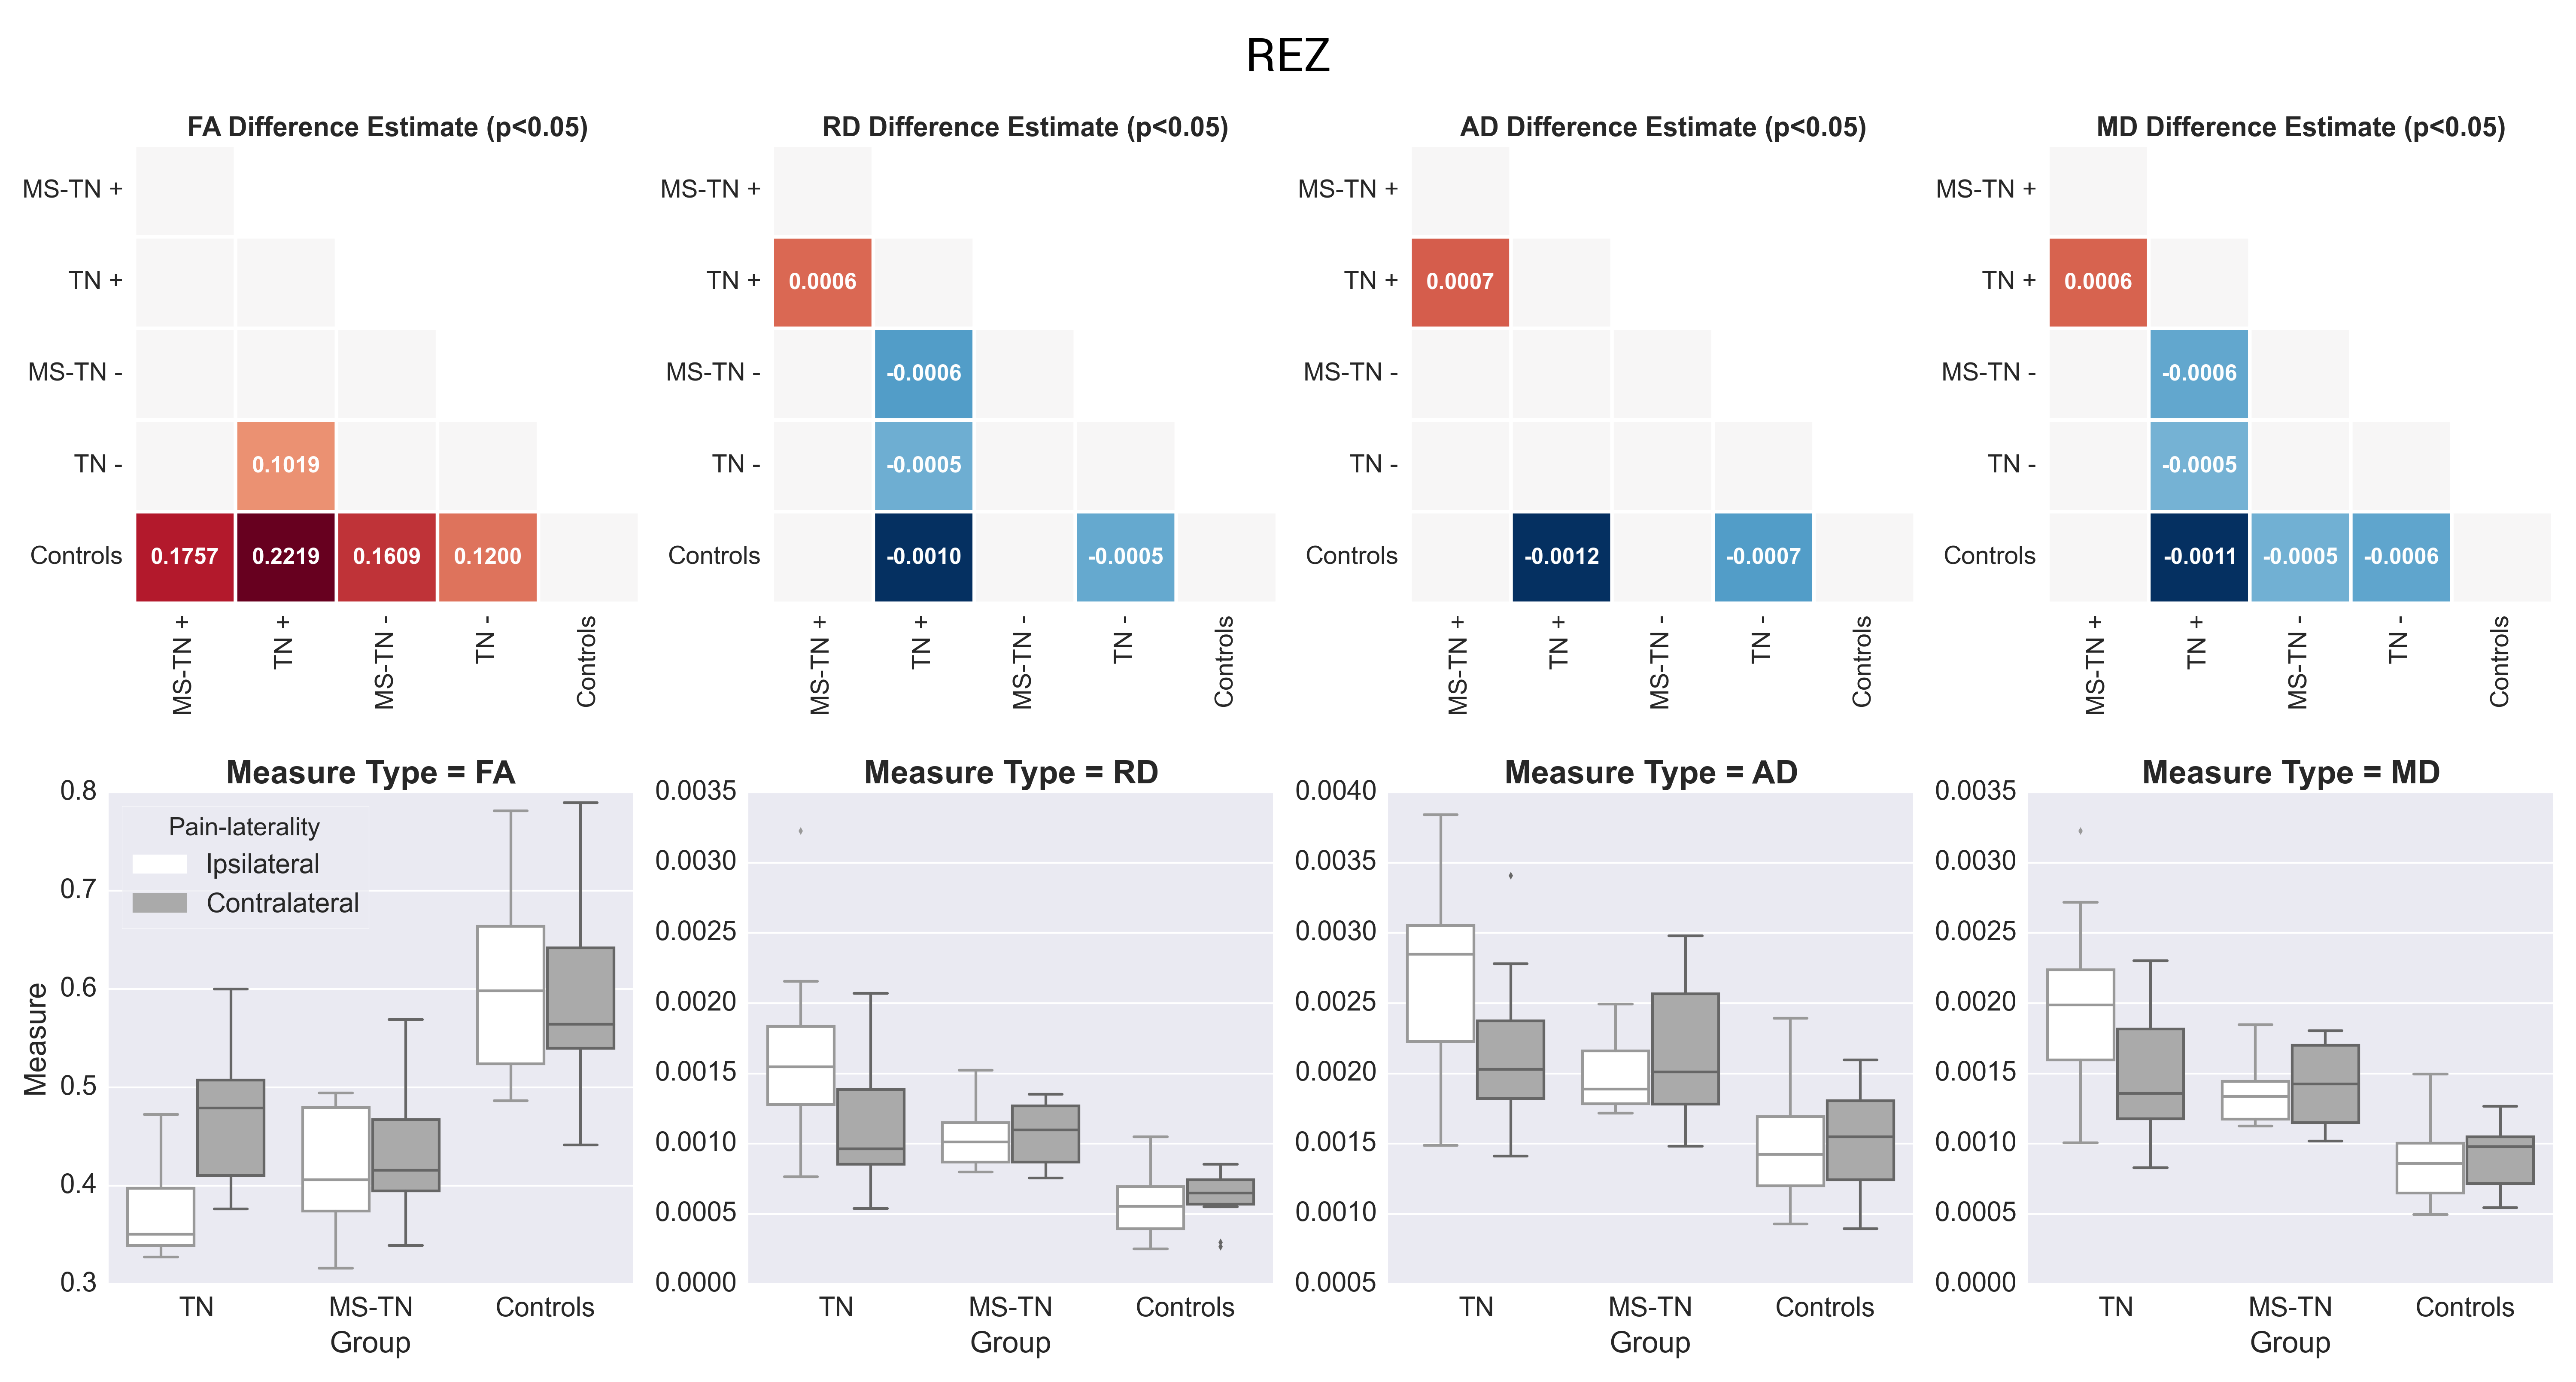
\includegraphics[width=\textwidth]{figure5.png}
\caption{In the REZ, MS-TN, and TN patients have significantly different diffusivities when compared to controls. TN+ also shows significantly different FA, RD, and MD from TN-. Moreover TN+ shows significant different from MS-TN+ as well. Please refer to Figure 4 for explanations of layout and annotations.}
\centering
\label{fig:MSfigure5}
\end{figure}

\begin{figure}[p]
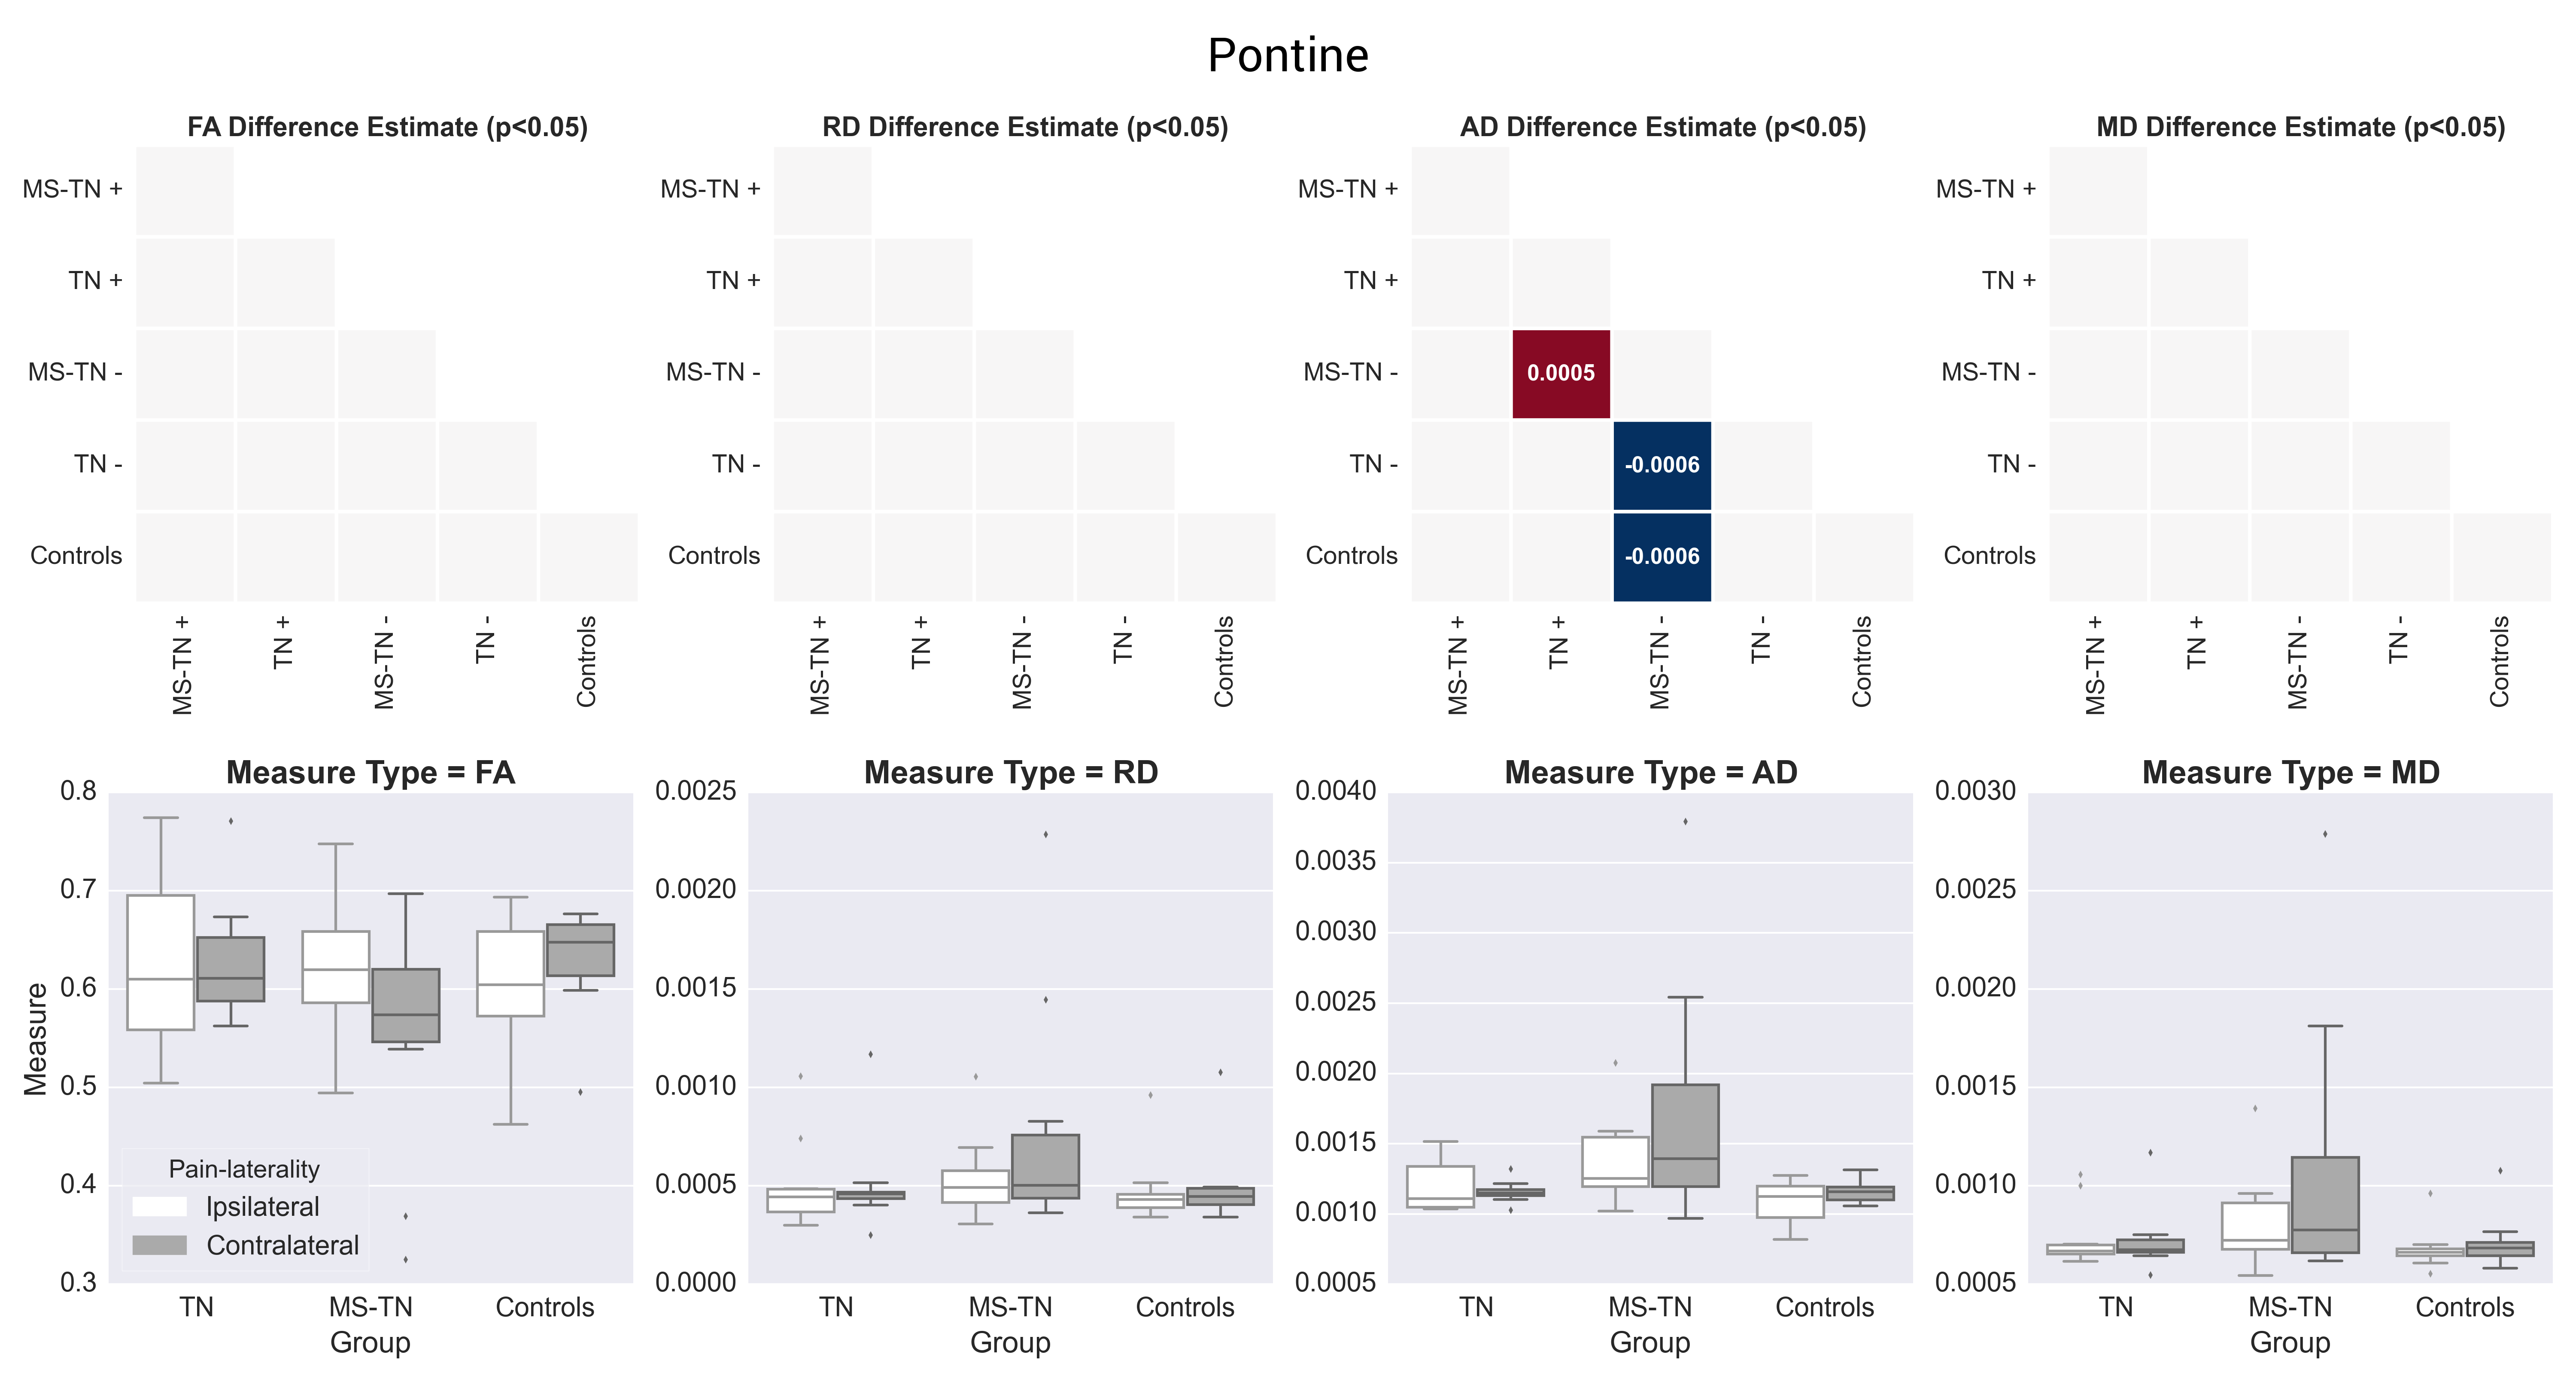
\includegraphics[width=\textwidth]{figure6.png}
\caption{In the pontine segment unaffected by MS plaques, there are little differences between groups. However MS-TN- shows significantly different AD than TN- and controls. Please refer to Figure 4 for explanations of layout and annotations.}
\centering
\label{fig:MSfigure6}
\end{figure}

\begin{figure}[p]
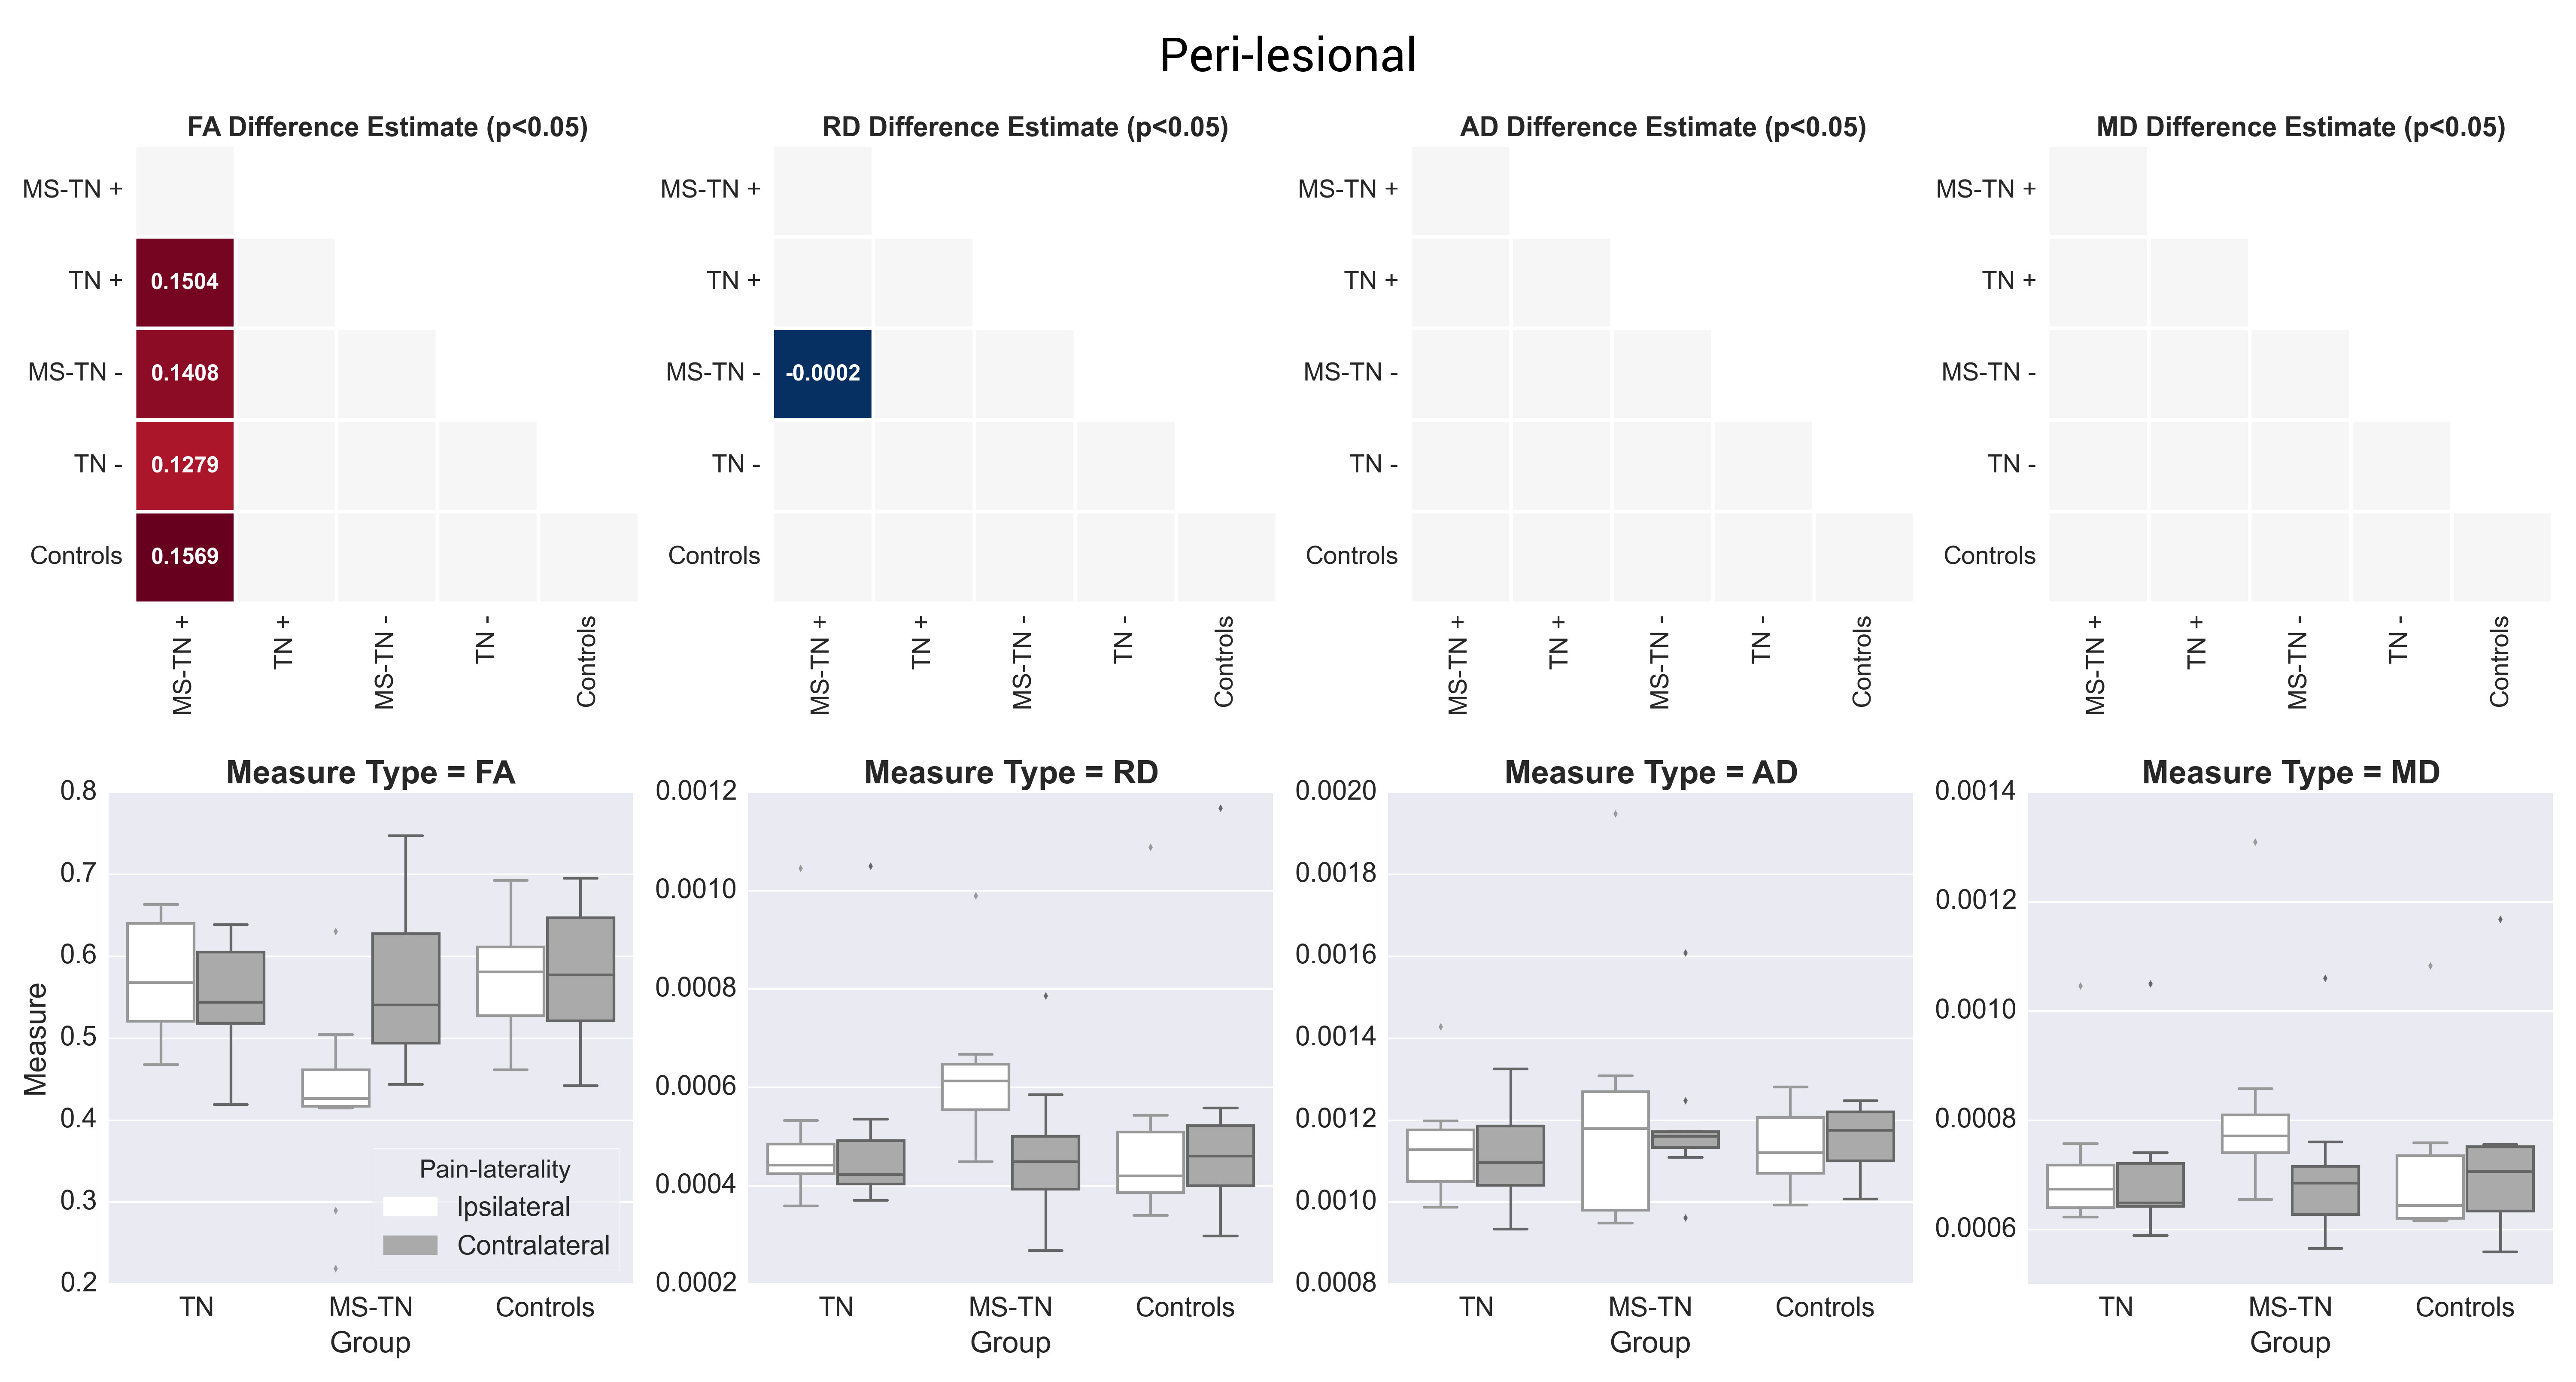
\includegraphics[width=\textwidth]{figure7.png}
\caption{The peri-lesional segment highlighting MS-TN+ specific diffusivity differences. Both MS-TN+ and MS-TN- show significantly lowered FA than all the other groups. RD of MS-TN- is also significantly lower than that of MS-TN+. Please refer to Figure 4 for explanations of layout and annotations.
http://msj.sagepu}
\centering
\label{fig:MSfigure7}
\end{figure}

\section{Discussion}

We demonstrate for the first time that diffusion MRI tractography is capable of anatomically distinguishing between TN and MS-TN. Analyses revealed unique, focal MS-TN diffusivity changes along CN V. These changes highlight the differences in diffusivities between MS-TN, TN and healthy controls, thereby permitting their use as neuroimaging signatures for distinguishing these conditions. 
Previous studies of the CN V with DTI tractography have been met with limitations of the single-tensor Gaussian diffusion model, and were incapable of resolving brainstem trigeminal tracts (Figure 2A). Recent improvements in multi-tensor imaging are now capable of more complex diffusion profile of crossing fibres in neural tissue, thereby permitting reliable reconstruction of the brainstem CN V (Figure 2B), and subsequently the study of CN V changes in MS patients (Figure 3). 

In patients with MS-TN we expected no changes in the extra-axial CN V segment, and that adverse changes to the CN V would be found in the intra-axial segment, within close proximity to the MS lesions. Conversely in TN patients, we expected CN V changes to be found within or near the extra-axial segment due to neurovascular compression. 

The results have agreed with our initial hypothesis. The coefficient matrices (Figures 4-7) revealed specific patterns demonstrating TN-specific diffusivity changes in the cistern and MS-TN-specific changes in the peri-lesional regions. In the TN REZ, FA changes are similar to the results found by DeSouza et al \cite{Desouza2013,Desouza2013c}, where the FA of the TN(+; pain-affected side) CN V is lower than that of TN(-; non-affected side). Additionally, while RD and MD changes in the TN REZ showed significant differences, no AD differences in the REZ were detected, suggesting that the nature of the diffusivity changes may be due to demyelination of the central myelin within the REZ. Interestingly, the cisternal TN(+) FA is demonstrably higher than the TN(-) segment, and also the cisternal FA of all other groups, suggesting that cisternal and REZ FA changes in TN are not homogenous along the nerve segment. Although there has been reports of hyperintensities in the cisternal CN V T$_{1}$ image with gadolinium contrast in MS \cite{VanderMeijs2002}, the lack of MS cistern findings in this study may be due to the limit of the sampled MS population. MS plaque locations are highly variable, and MS-TN patients were not filtered specifically for cistern region plaques. 

Diffusivity disruptions of CN V in MS-TN patients are likely due to MS plaques at the regions proximal to the main sensory nucleus. While AD has been associated with neurological disruptions in MS \cite{Budde2009,Kim2006}, the present study showed a lack of change in AD. This may relate to the observation that we did not select subjects based on their disease severity, but based on their pain. Disease severity was in fact variable in this group. Future studies will be able to address this point in more detail, by taking into account other MS manifestations in addition to pain, and correlation with diffusion metrics. Lower REZ FA in MS-TN compared to controls suggests that global neural tissue diffusivity in MS-TN is significantly different from that of healthy controls. Similar findings can be seen in the pontine region, where only the MS-TN AD measures are distinctly different from the other groups. However while AD is commonly correlated with axonal integrity, the high concentration of crossing fibres in the pontine region may introduce confounds into these correlations. Improvements in diffusivity metric measurements in such tissues are needed to further understand these findings. 

\subsection{Limitations and future directions}
The study aimed to demonstrate that diffusion MRI can detect localized CN V differences in MS-TN, and to evaluate the feasibility of this novel approach in a group of patients. Therefore we did not explore the course of MS disease progression and other details in the MS-TN patient group in this study. However it has demonstrated that by utilizing MTT to not only visualize, but also to assist in nerve segmentation and statistical analysis, more complete insights into the changes of white matter anatomy can be gained. We have found that peripheral CN V does not change homogeneously in pathology. Other white matter pathways are also likely to be differentially affected in varying segments in other pathological states such as MS. 

With this approach, future longitudinal studies may reveal more about white matter changes and associated pain, cognitive, and motor-related measures across the disease’s progression. Moreover, this strategy may allow for pre- and post-treatment predictions in white matter changes, ultimately aiding in clinical prognostication and the identification of high-risk subjects. Therefore, this study paves the way for a more systematic approach to the understanding of pain and white matter anatomy using non-invasive neuroimaging techniques.

\section{Conclusion}
The study demonstrates that MS-TN and TN have differentially localized pathophysiology at the level of CN V in the brainstem. MS plaques disrupt the diffusivity of brainstem CN V fibres near the CN V nucleus, while TN diffusivity disruptions are focused on the cistern and REZ segments. The regions affected by MS and TN REZ suggest changes in myelination of the affected CN V segment. Using this imaging technique, TN and MS-TN can be distinguished by unique localized diffusivity changes in the different CN V segments.